\documentclass[twoside,twocolumn,8pt]{extarticle}


% ------
% Fonts and typesetting settings
\usepackage[sc]{mathpazo}
\usepackage[T1]{fontenc}
\linespread{1.05} % Palatino needs more space between lines
\usepackage{microtype}


% ------
% Page layout
\usepackage[hmarginratio=1:1,top=10mm,columnsep=20pt,left=0.8in, right=0.8in]{geometry}
\usepackage[font=it]{caption}
\usepackage{paralist}
\usepackage{multicol}

% ------
% Lettrines
\usepackage{lettrine}


% ------
% Abstract
\usepackage{abstract}
	\renewcommand{\abstractnamefont}{\normalfont\bfseries}
	\renewcommand{\abstracttextfont}{\normalfont\itshape}


% ------
% Titling (section/subsection)
\usepackage{titlesec}
\renewcommand\thesection{\Roman{section}}
\titleformat{\section}[block]{\large\scshape\centering}{\thesection.}{1em}{}

\usepackage{graphicx}
% ------
% Header/footer


\usepackage{fancyhdr}
\pagestyle{fancy}

\setlength\headheight{90.0pt}
\addtolength{\textheight}{-90.0pt}

\fancypagestyle{firststyle}
{
   	\fancyhead[L]{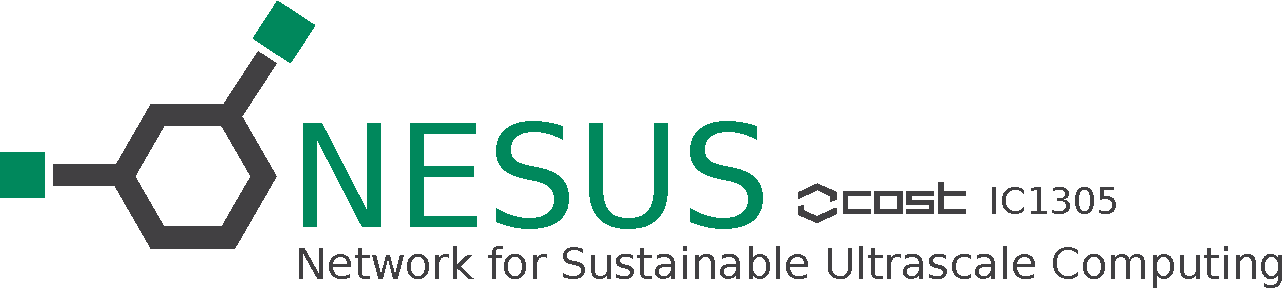
\includegraphics[height=5.5em]{pictures/nesus.pdf}}
	\fancyhead[C]{}
	\fancyfoot{}
	\fancyhead[R]{\small{Book paper template $\bullet$ October 2016 $\bullet$ Vol. I, No. 1}}
	\fancyfoot[RO,LE]{\thepage}
}
	\fancyhead[R]{}
	\fancyhead[L]{}
	\fancyfoot{}
	\fancyhead[C]{\small{Book paper template $\bullet$ October 2016 $\bullet$ Vol. I, No. 1}}
	\fancyfoot[RO,LE]{\thepage}


% ------
% Clickable URLs (optional)
\usepackage{hyperref}

% ------
% Maketitle metadata
\title{\vspace{-10mm}%
	\fontsize{24pt}{10pt}\selectfont
	\textbf{Modeling Emerging Complex Memory Hierarchies With The Roofline Model}
	}
	
		
\author{%
	\large
	\textsc{Nicolas Denoyelle \and Aleksandar Ilic} \\[2mm]
	\normalsize{	Inria - France -- INESC-ID -- Portugal}\\
	\normalsize{	\href{mailto:Nicolas.Denoyelle@inria.fr}{Nicolas.Denoyelle@inria.fr} \href{mailto:ilic@sips.inesc-id.pt}{ilic@sips.inesc-id.pt}}
	\vspace{-5mm}
	}

\date{}

\providecommand{\keywords}[1]{\textbf{\textit{Keywords}} #1}

%%%%%%%%%%%%%%%%%%%%%%%%
\begin{document}



\twocolumn[
  \begin{@twocolumnfalse}

%\maketitle

\thispagestyle{firststyle}


\begin{abstract}
\noindent The ever growing complexity of high performance computing systems imposes significant challenges to exploit as much as
  possible their computational and communication resources.
  Recently, the Cache-aware Roofline Model has has gained popularity due to its simplicity modeling multi-cores with complex memory
  hierarchy, characterizing applications' bottlenecks, and quantifying achieved or remaining improvements.
  In this short paper we push this model a step further to model NUMA and heterogeneous memories with a handy tool, and spot data
  locality bottlenecks on such systems.
\end{abstract}


\keywords{Roofline Model, heterogeneous memory, NUMA, Cache}

 \hrulefill
\bigskip 


\end{@twocolumnfalse}
]


\section{Introduction}\label{sec:Intro}
%+++++++++++++++++++++++++++
Emerging memory technologies (e.g heterogeneous memory architectures with non-volatile memory, on-package memory \dots), are
required to address applications' needs and improve the performance at the cost of a growing hardware complexity.
The memory wall makes memory management one of the main bottlenecks, and the variety expansion of allocable memories will
definitely make data locality a performance hot spot, even on single chips.

We think we can leverage the Roofline Model to detect the latters accross on-chip's memories.
For instance, a data allocated on low-bandwidth memory, may lead the application to become bandwidth bound.
Our extension to heterogeneous and NUMA memory of the Cache Aware Roofline Model shows that in such sytems,
memory bandwidth may vary from one pair (Core, memory) to another.
Thus memory bound applications with bad data locality can be spotted by observing their performance variation beeing similar to
memories performance differences.

In our contribution, we developped a handy tool to build and validate the model on such systems.

The remainder of this paper is organized as follow:

The section~\ref{sec:state_of_art} will describe the Roofline Model and its main technical variations.
Finally section~\ref{sec:contrib} will briefly describe our implementation to measure memory bandwidths, and validate the model.

\section{The Roofline Model Then and Now}\label{sec:state_of_art}
%+++++++++++++
\begin{figure}
  \centering
  \includegraphics[width=.2\textwidth]{pictures/model_drawing}
  \caption{Roofline model draw}
  \label{fig:roofline_draw}
\end{figure}

The original paper~\cite{Williams:2009:RIV:1498765.1498785} depict a machine with two subsystems: a memory and a compute unit,
executing the instructions dispatched from a common instruction channel.

This idea is drawn on figure~\ref{fig:roofline_draw}.
Depending on the operational intensity (i.e. the ratio of compute instructions (blue rectangles) over memory instructions (green rectangles)),
one unit, the other or both may be saturated with instructions. The width of the memory channel is the bandwidth and the width
of the compute channel is the floating point peak (fpeak) performance. The model assumes there can be no dependency between
instructions (they can overlap perfectly) and instructions' lattency is hidden.

On figure~\ref{fig:orig_model} is shown the graphical representation of the model.
The operational intensity stands on abscissa and the performance stands on the ordinate axis.
Top horizontal lines show the fpeak performance for different type of compute instructions and
oblique lines show the memory bandwidth for different types of memories. On this representation
one can see that: the roofline model ($min(bandwidth*operational\_intensity, fpeak)$) shows whether a pattern of compute/memory
instructions interleaving is either compute or memory bound if the maximum achievable performance is bound whether by the fpeak
performance or the bandwidth.

The model has been successfully used in
several~\cite{Kim20111201}~\cite{Rossinelli2164}~\cite{vanNieuwpoort:2009:UMH:1542275.1542337} applications optimizations, whether
to prove bottlenecks, or measure achievable (or achieved) improvements.

It has been applied to other memory subsystems~\cite{ilic2014cache}, energy~\cite{7493653}, and abstract runtime systems.

Based on the Cache Aware Roofline Model~\cite{ilic2014cache} methodology, we applied and validated the model to heterogeneous
memory subsystems.

\section{Contribution}\label{sec:contrib}
%+++++++++++++
\begin{figure*}
  \centering
  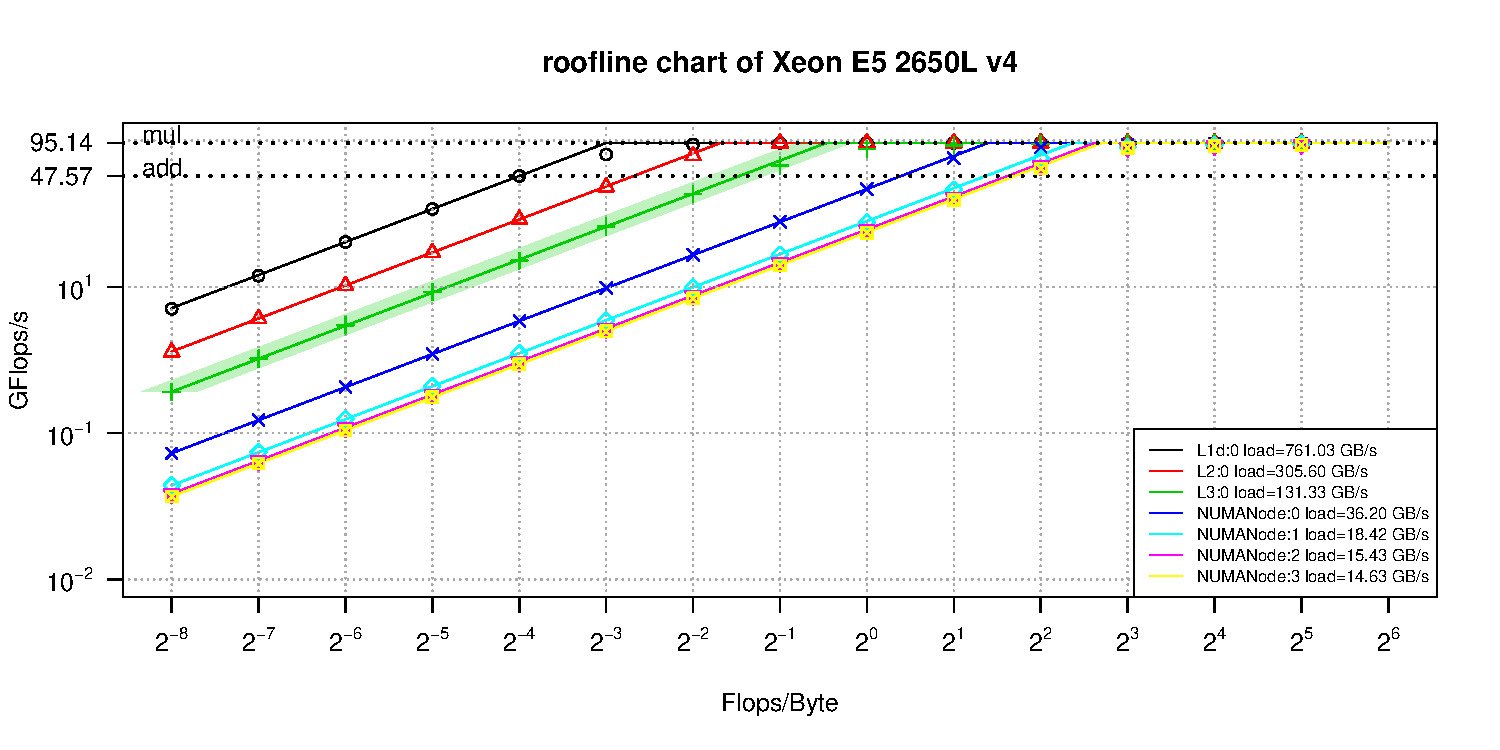
\includegraphics[width=\textwidth]{pictures/roofline_model}
  \caption{The roofline chart on a Xeon E5 2650L v4 processors with 4 NUMA memories spreads on two different packages. On ordinate, the performance is in $10^{^9}$ floating point operations per second. On abscissa, operational intensity is the number of floating point operations per bytes loaded.}
  \label{fig:orig_model}
\end{figure*}

In our contribution, we developped a tool able to benchmark rooflines and validate them with micro kernels, compatible with intel
chips.

Each benchmark (rooflines, and validation) is made of assembly code using best architectures instructions available at compile
time.

In brief, the fpeak benchmark repeats compute instructions and outputs $\frac{n*iFlops}{time}$ where $n$ is the number of compute
instructions and $iFlops$ is the number of floating point operations computed per instruction.

The bandwidth benchmark repeats coallesced memory accesses on a private\footnote{Each thread have its own buffer's chunk} buffer of several sizes fitting the memory to benchmark and outputs $\frac{n*iBytes}{time}$ where $n$ is the number of memory instructions and $iBytes$ is the number of Bytes transferred per instruction.

And the validation kernels interleave previously defined benchmarks instructions and output its performance and operational intensity.

We can find several arithmetic floating point operation peaks (addition, multiplication, overlapping multiply add, and fuse
multiply add), as well as several bandwidth types (load, store, non temporal load, non temporal store, interleaving of 2 loads and one store), and for several memory levels (L1, L2, L3, (caches \dots), NUMA memories, MCDRAM \dots) detectable with hwloc~\cite{6903671} library.

\begin{figure}
  \centering
  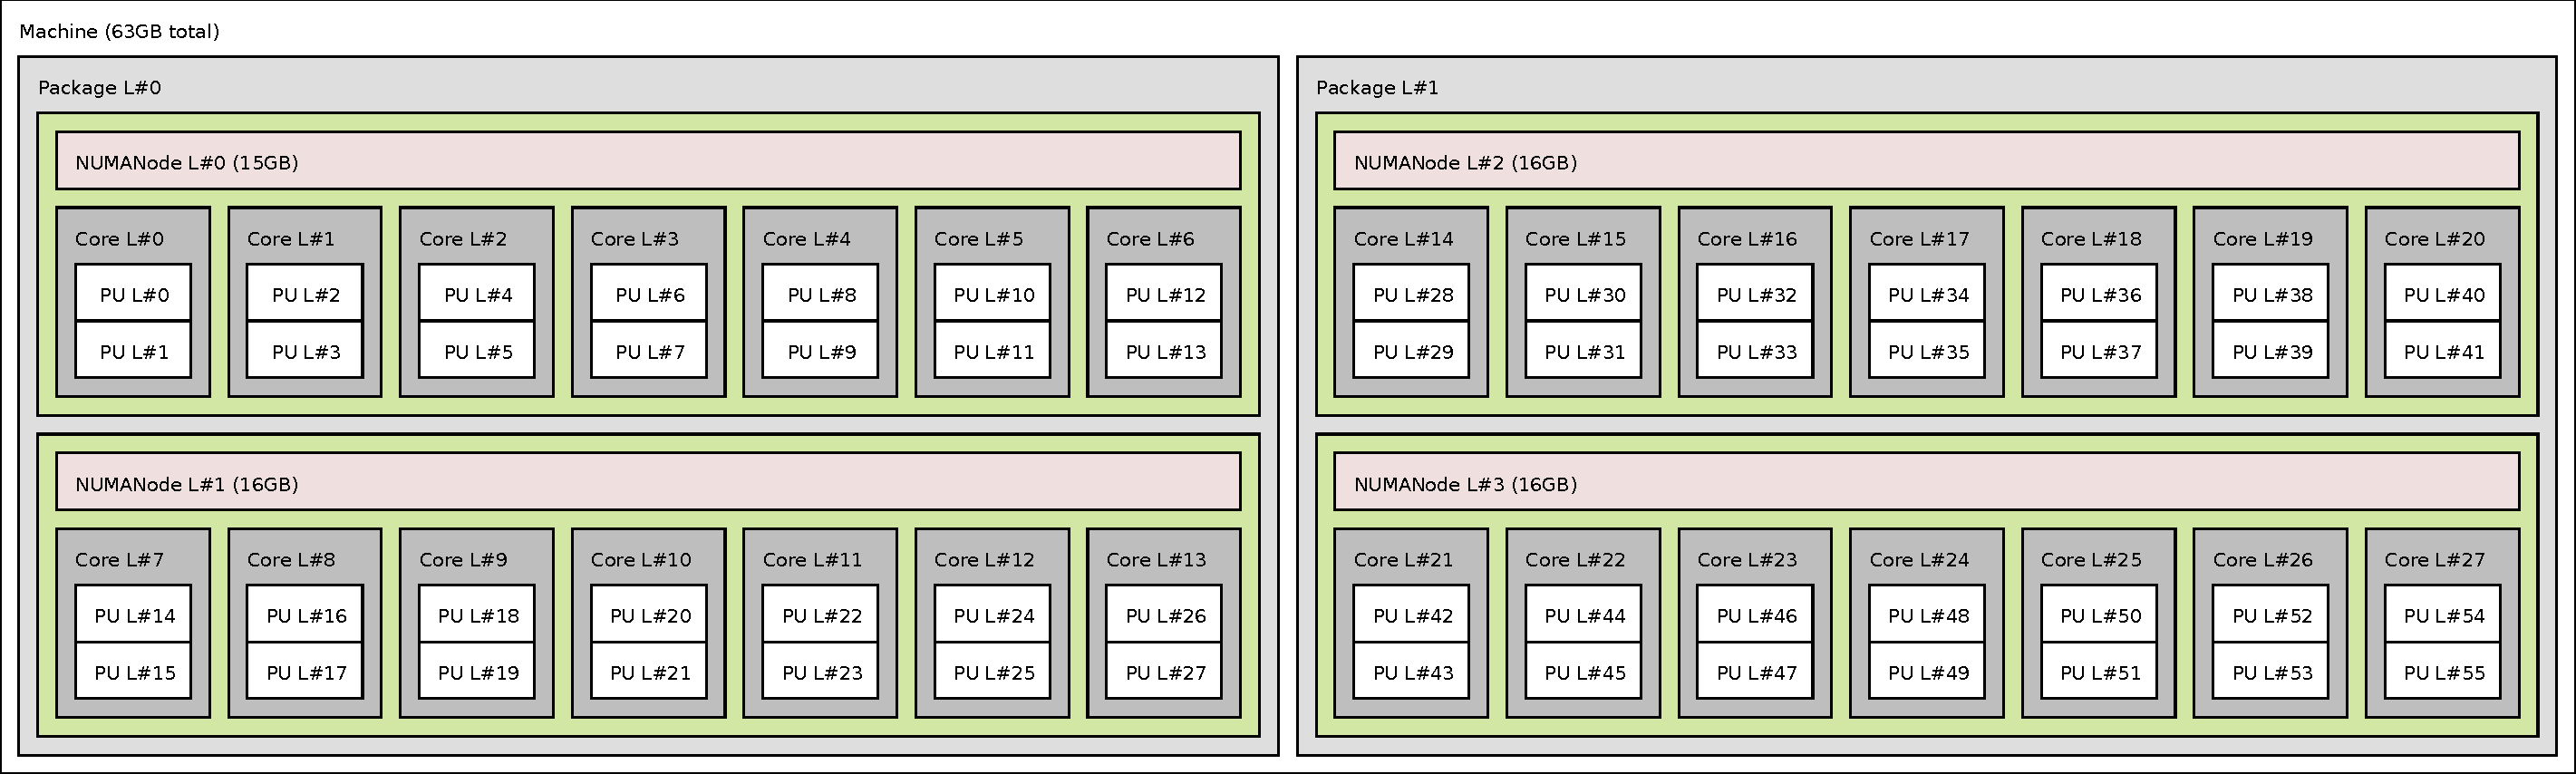
\includegraphics[width=.5\textwidth]{pictures/Xeon_E5_2650L_v4}
  \caption{Machine topology, with hidden caches}
  \label{fig:joe0}
\end{figure}

Figure~\ref{fig:joe0} shows a model of such a machine given by hwloc.
Nested boxes represent hierarchical inclusiveness of ressources in the machine.
Our benchmark can work both in sequential and in parallel.
In the former, one benchamrk thread is spawn on first Core (left most) of the machine.
In the latter, one benchmark thread per Core of the first NUMA memory node is spawn, and threads measure (Flops and Bytes) are
accumulated.
The parallel model representation obtained from machine~\ref{fig:joe0} is shown on figure~\ref{fig:orig_model}.
The system yields a load bandwidth of 761GB/s for the total of its 7 L1 caches per Node, whereas the shared local memory
(NUMANode:0) yields a bandwidth of 36GB/s for the same type of micro-operations.
Remote memories' bandwidth are obtained by running the same benchmark as local memory, but explicitly allocating the data on remote
 memories.
On figure~\ref{fig:orig_model}, the lines shows the top measures.
One can notice, on L3 a wider line with less opacity showing the measured bandwidth deviation.
For each memory we use different sizes of buffers fitting the memory, and depending on the buffer size, the bandwidth may vary.
We can also notice that for L1 (black line), the points does not stick very well to lines around the ridge. Actually the points
does not measure the bandwidths, but instead validate rooflines. They consist of micro-benchmarks of different known operational
intensities, interleaving memory and compute instruction to reach rooflines, and show how realistic the model is with those
metrics, by measuring each micro-benchmark's performance.

\section{Conclusion and future work}\label{sec:conclusion}
%+++++++++++++++++++++++++++++++++++
In this short paper we prestented the Roofline Model and an extension to heterogeneous memory's sytem using the Cache Aware
Roofline Model methodology. Later on we will validate the interest of this representation with applications. 

\bibliographystyle{plain}
\bibliography{references}

\end{document}
